\begin{frame}{Navier-Stokes}
  \begin{columns}
    \begin{column}{0.45\textwidth}
      \begin{figure}
        \begin{flushleft}
          {\setlength{\unitlength}{\textwidth}
            \begin{picture}(1,1.5)(0,0)
              \put(0.0,0.75){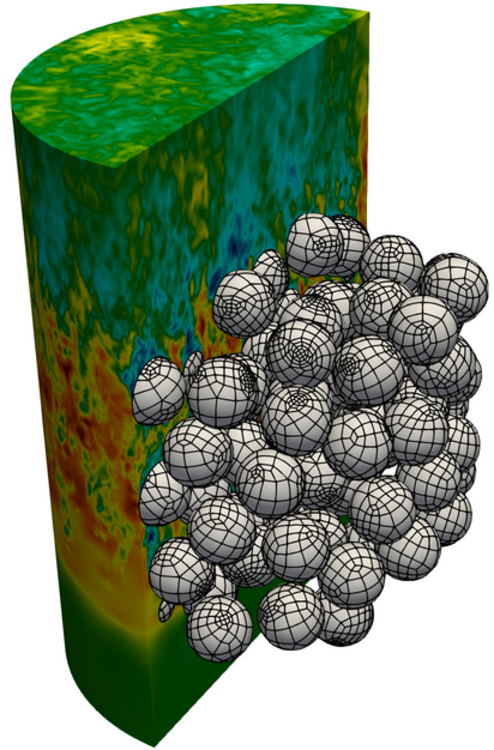
\includegraphics[width=0.45\textwidth, left]{../figs/pb146.png}}
              \put(0.5,0.75){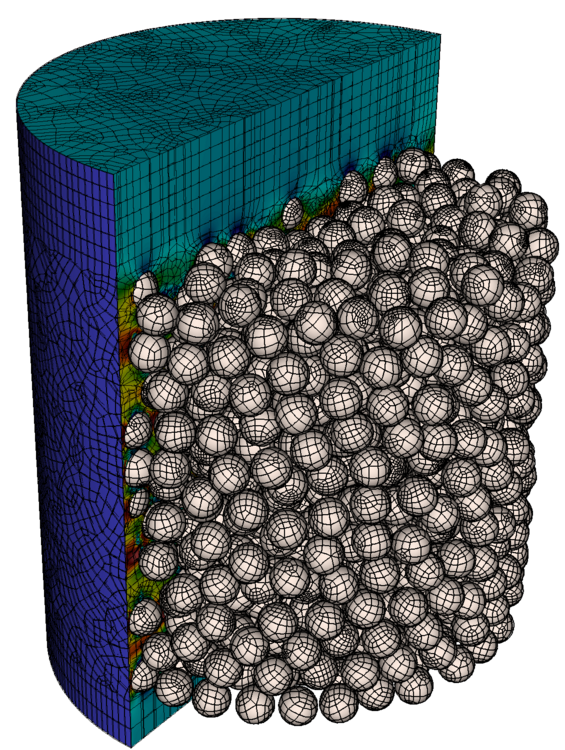
\includegraphics[width=0.5\textwidth, left]{../figs/pb1568.png}}
              \put(0.0,0.40){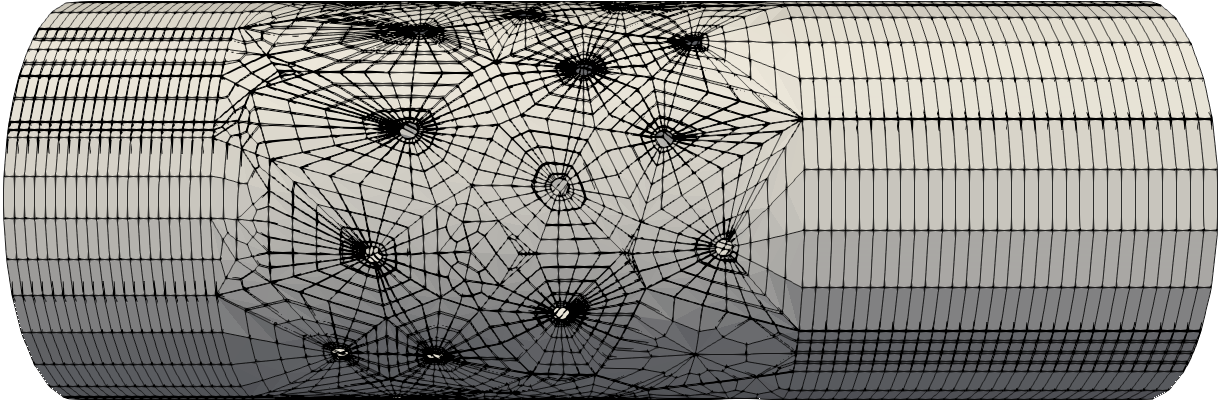
\includegraphics[width=0.9\textwidth, right]{../figs/peb67-side-profile.png}}
              \put(0.0,0.00){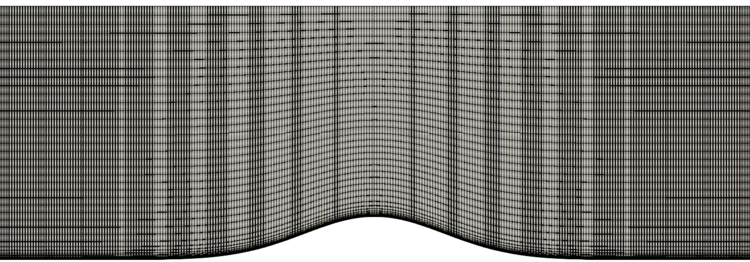
\includegraphics[width=0.9\textwidth, right]{../figs/BoeingSpeedBump.png}}

              \put(-0.05,0.80){\large (a)}
              \put(0.40,0.80){\large (b)}
              \put(-0.05,0.45){\large (c)}
              \put(-0.05,0.05){\large (d)}
  
            \end{picture}}
        \end{flushleft}
      \end{figure}
    \end{column}
    \begin{column}{0.55\textwidth}
      \begin{table}\tiny
\begin{tabular}{||c| c c c ||}
  \hline
  Case Name & $E$ & $p$ & $n$\\
  \hline\hline
  146 pebble  (a) & 62K & 7 & 21M\\
  1568 pebble (b) & 524K & 7 & 180M\\
  67 pebble   (c) & 122K & 7 & 42M\\
  Speed bump  (d) & 885K & 9 & 645M\\
\hline
  & CFL & $\Delta t$ & $T_{restart}$\\
  \hline \rule{0pt}{2.5ex} 
  %(a) \footcite{lan_all-hex_2021} & 4 & $2\times 10^{-3}$ & 10\\
  %(b) \footcite{lan_all-hex_2021} & 4 & $5\times 10^{-4}$ & 20\\
  %(c) \footcite{yuan2020spectral} & 4 & $5\times 10^{-5}$ & 10.6\\
  %(d) \footcite{shur_direct_2021} & 0.8 & $2\times 10^{-3}$ & 5.6\\
  (a) & 4 & $2\times 10^{-3}$ & 10\\
  (b) & 4 & $5\times 10^{-4}$ & 20\\
  (c) & 4 & $5\times 10^{-5}$ & 10.6\\
  (d) & 0.8 & $2\times 10^{-3}$ & 5.6\\
  \hline
  & $Re$ & Tol & Steps \\
  \hline \rule{0pt}{2.5ex} 
  (a) & $5000$ & $10^{-4}$ & 2000\\
  (b) & $5000$ & $10^{-4}$ & 2000\\
  (c) & $1460$ & $10^{-4}$ & 2000\\
  (d) & $10^6$ & $10^{-5}$ & 2000\\
  \hline
\end{tabular}
\captionsetup{labelformat=empty}
\caption{
  \small
  %Problem discretization, timestepping parameters.
  %Pebble cases use a two stage subcycling scheme.
  %All cases use a 2nd-order timestepper with 10 prior solution vectors
  %to generate the initial guess%. \cite{fischer_projection_1998}.
  \label{table:problem-sizes}
}
\end{table}
    \end{column}
    \end{columns}
\end{frame}